\documentclass[]{article}

\usepackage{multirow,hhline,graphicx,array}
\usepackage{makecell}
\usepackage{geometry}
\usepackage{pdfpages}
\usepackage{titlesec}
\usepackage{float}
\usepackage{caption2}
\usepackage[hidelinks]{hyperref}

\makeatletter
\def\@maketitle{%       
	\newpage
	\null
	\vskip 14em%
	\begin{center}%
		\let \footnote \thanks
		{\LARGE \@title \par}%
		\vskip 12em%
		{\large
			\lineskip .5em%
			\begin{tabular}[t]{c}%
				\@author
			\end{tabular}\par}%
		\vskip 1em%
		{\large \@date}%
	\end{center}%
	\par
	\vskip 1.5em}
\makeatother
%opening
\title{\Huge COP5725 - Database Management Systems\vspace{2.8em} \LARGE \textbf{Project Deliverable 2:} Weather Recording System}
\author{
	\Large Group 19:\qquad He,Jiahui,\\
	\Large \qquad\qquad\qquad\qquad Shi,Qinxuan,\\
	\Large \qquad\qquad\qquad\qquad Wang,Shihuan,\\
	\Large \qquad\qquad\qquad\qquad\qquad Zhang,Guanglong
}
\date{}
\special{papersize=8.5in,11in}
\geometry{left=2.5cm,right=2.5cm,top=1.5cm,bottom=1.5cm}


\begin{document}
	
	\maketitle
	\clearpage
	
	\tableofcontents
	\clearpage
	
	\section{Quality of the overview and description of the application}
	
	Weather and climate are important factors that determine the normal operation of all sectors of society. Weather usually describes the atmospheric conditions at a certain point or period of time, such as temperature, precipitation, humidity, wind, and ultraviolet index. Weather data is very important in our daily lives. People change their clothes and daily travel plans according to changes in weather and climate. The collected precipitation and temperature data can be used to prevent natural disasters or disasters such as floods and droughts. In addition, weather and climate play a decisive role in agriculture and aviation. For example, weather conditions determine whether an aircraft can take off on time and which route is the safest and safest to choose. At the same time, the construction industry also needs weather data to arrange construction plans and programs. The long-term collection of weather data is of great significance for summarizing the meteorological conditions of the region and predicting the climate change trend in the region. \\
	
	\noindent Nowadays, there are many ways to collect weather data, from large weather radars to small weather stations, which are recording weather data all the time. In view of the importance of weather data, how to properly process and utilize these data has become an important topic. However, using paper data to record and analyze weather data is very cumbersome, inefficient, and unreliable. In addition, the paper-based data recording method is not convenient for storage and quick query. Therefore, we use the Oracle database to design a Weather Recording System. \\
	
	\noindent With the help of a web-based user interface, the system can store these large amounts of weather data in a structured manner and display these data publicly. For different users, you can use this system to operate on weather data according to different needs. In addition, the administrator can also update the data. This database system makes it possible to store a large amount of weather data with high security and long-term storage and at the same time improve the ease of use of the data. \\
	
	\noindent Here is the descripton of the system. The weather recording system needs users to sign up or login to the system. Our system also has an administrator accout to manage users. To the fuctions that showing the data: firstly, Our system will show the basic weather data like temperature, precipitation and so on in the form of table, and users could choose the time period as well as the cities to get the data they want. The second function is that users can know about the information of the weather stations and cities from which our system get the weather data from. What's more, we have five interesting and complex trend queries which will be described in detail in section 2. Users will get the information that is derived from the basic data to be showed in different kinds of charts, for example, they can learn about the change of temperature over a long time period or compare the precipitation at different cities during the same year. 
	
	\clearpage
	
	\section{Quality of the user interface design including the application-specific network or graph of web pages and the  integration of the complex trend queries}
	
	\subsection{Design of the application-specific network}
	
	The system is started from the web page of login, which is showed in the Figure 1. Then, we have three different conditions. The first is when the account that entered is administrator, the system will go to the page that is particularly designed for the administrator to manage all the user. At userManage page, the administrator can delete user, modify user information (Administrator is not allowed to change user's password) or check out the statistics of the number of new user. The second condition is that when the user needs to sign up and create a new account, the system will be directed to the page which is designed for creating new account. At this page, the user only need to enter username and password to create a new account, and after the creation, the web page will direct to the welcome page automatically. The third condition is the most common condition, the user login with his/her username and password correctly, then they will see the welcome page. We currently decide to use the temperature data form of basic data to be the welcome page of out system. The welcome page has several fuctions, users can get to the basic data page, station information page, city information page and trend queries page. Exactly, we are going to put all these parts in a side-menu, so that the users can get to each part from every page. What's more, users can also click on the sign of head portrait and go to the userInfo page at which users could change their names and passwords. After making sure to change, the administrator will get the notice of change.
	
	\begin{figure}[H]
		\centering
		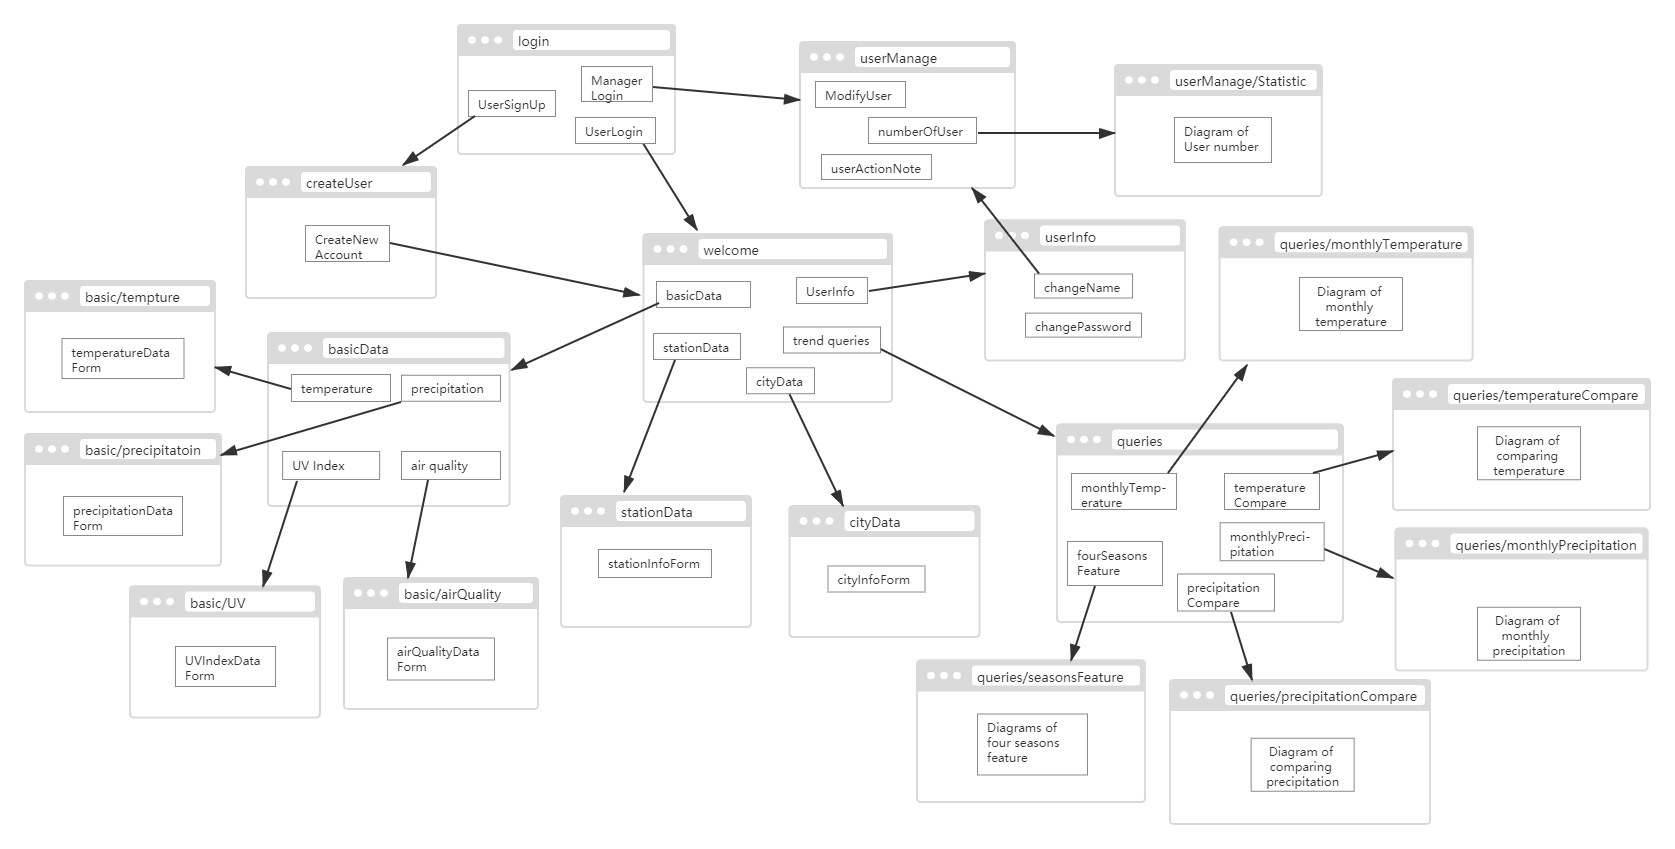
\includegraphics[width=1.1\linewidth]{../network}
		\caption{application-specific network}
		\label{fig:network}
	\end{figure}
	
	\clearpage
	
	\subsection{Design of each web page}
	
	\noindent Users and administrators enter their username and password to log in to the weather recording system.
	\begin{figure}[H]
		\centering
		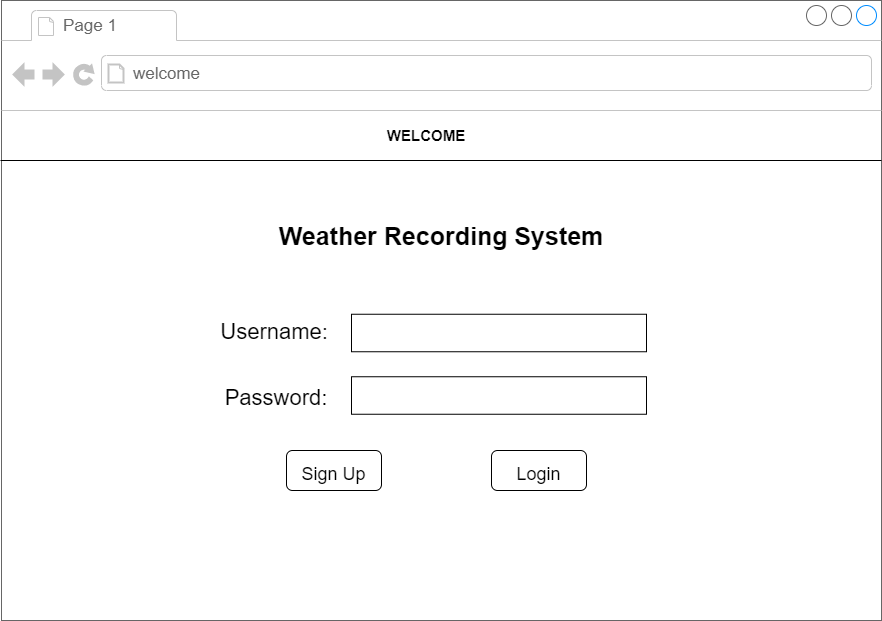
\includegraphics[width=0.82\linewidth]{../login}
		\caption{Login}
		\label{fig:login}
	\end{figure}
	
	\noindent After logging into the account, the administrator can receive messages from users, thus adding and modifying user information. To facilitate the operation, the administrator can use the complex query function for user information.
	\begin{figure}[H]
		\centering
		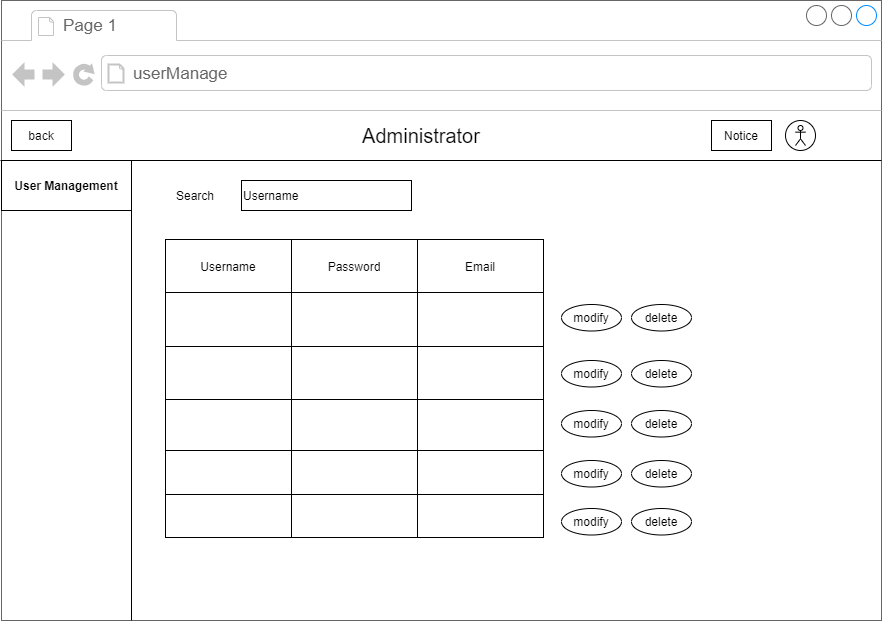
\includegraphics[width=0.82\linewidth]{../userManage}
		\caption{User Manage}
		\label{fig:usermanage}
	\end{figure}
	
	\noindent If the user does not have an account, click the 'Sign Up' button. Jump to the registration page, and enter the username, password and email to sign up.
	\begin{figure}[H]
		\centering
		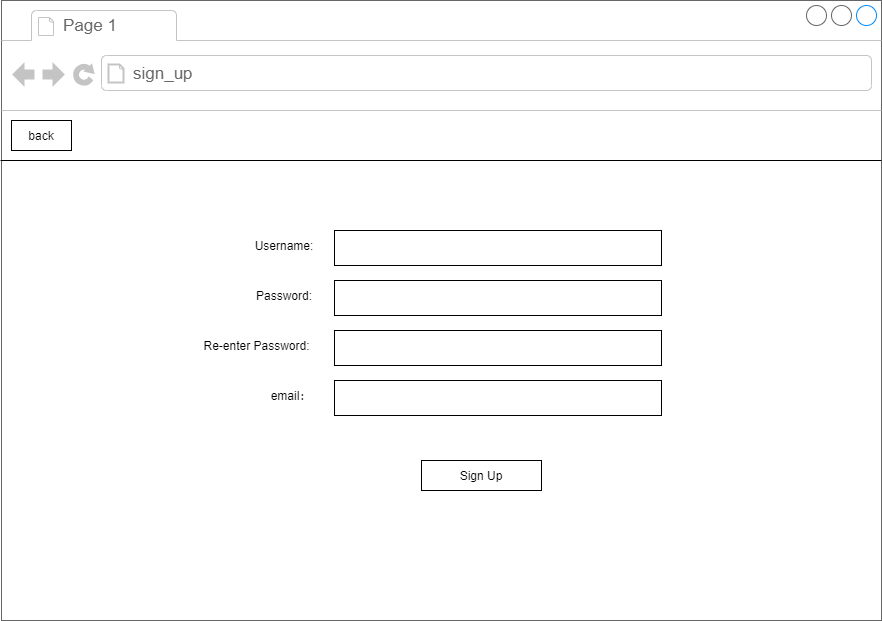
\includegraphics[width=0.83\linewidth]{../signUp}
		\caption{Sign Up}
		\label{fig:signup}
	\end{figure}
	
	\noindent The administrator can choose the from time and to time, then the diagram will show the number of new users who sign up to the system over the time period.
	\begin{figure}[H]
		\centering
		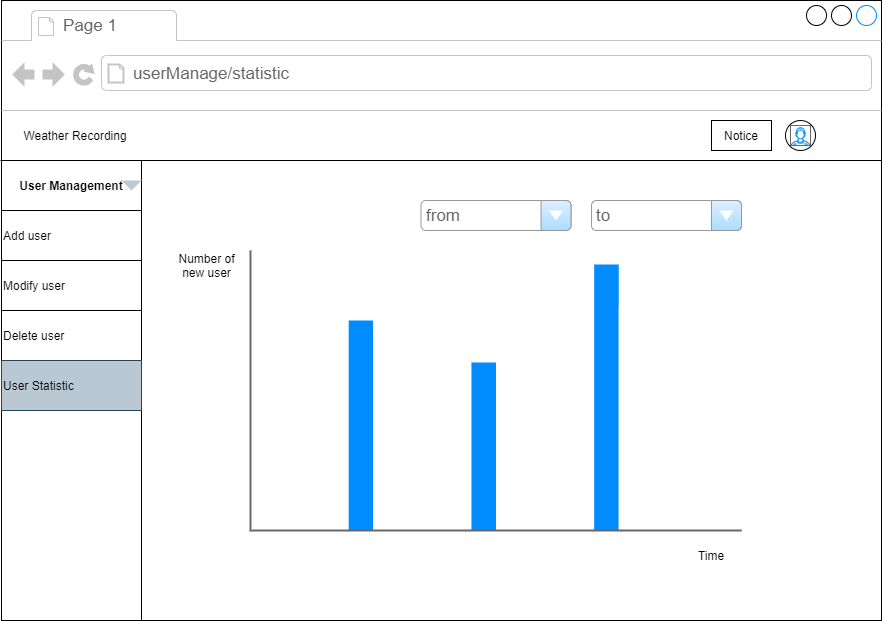
\includegraphics[width=0.85\linewidth]{../userManage-statistic}
		\caption{userManage/statistic}
		\label{fig:usermanage-statistic}
	\end{figure}
	
	\noindent After clicking the sign of head portrait, the users can go to the page of userInfo and change their name and password. They could also go back by clicking the back button.
	\begin{figure}[H]
		\centering
		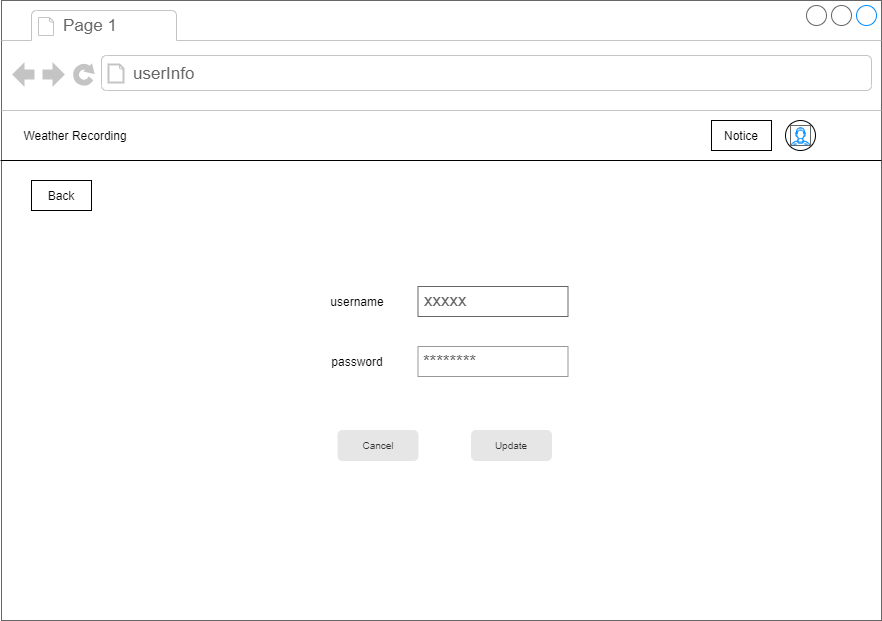
\includegraphics[width=0.85\linewidth]{../userInfo}
		\caption{userInfo}
		\label{fig:userinfo}
	\end{figure}
	
	\noindent The web page of temperature data of basic data part, which is also the welcome page of the system. We will show the default data in the form, and the users can choose the from and to time as well as cities to get the data they want. The system also support keyword search.
	\begin{figure}[H]
		\centering
		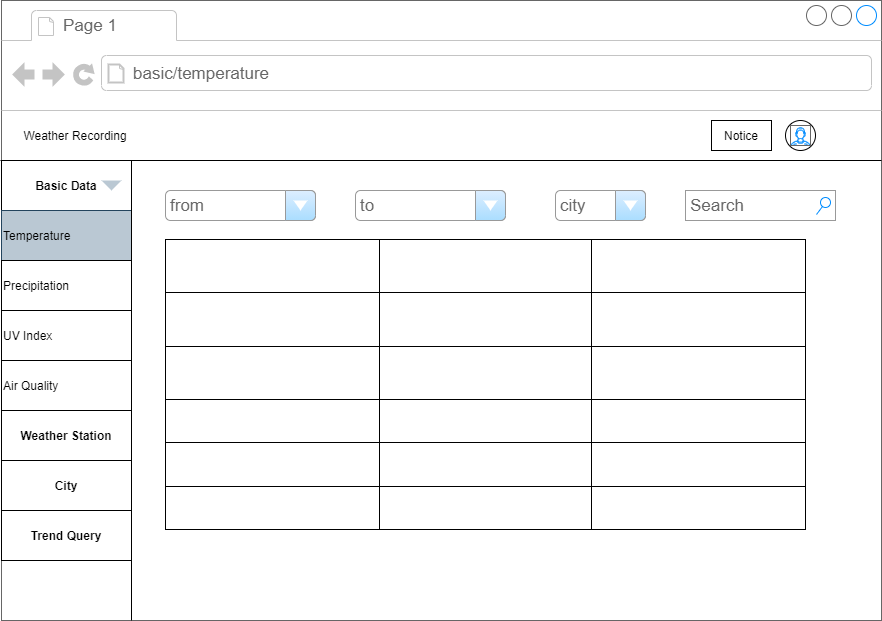
\includegraphics[width=0.8\linewidth]{../basic-temperature}
		\caption{basic/temperature}
		\label{fig:basic-temperature}
	\end{figure}

	\noindent The other part of basic data, precipitation data, UV Index data and air quality data, their web pages look almost same as the temperature data, so we are not going to show these pages in detail. \\
	
	\noindent The station information web page can tell users about information of the weather stations from which we get the weather records.
	\begin{figure}[H]
		\centering
		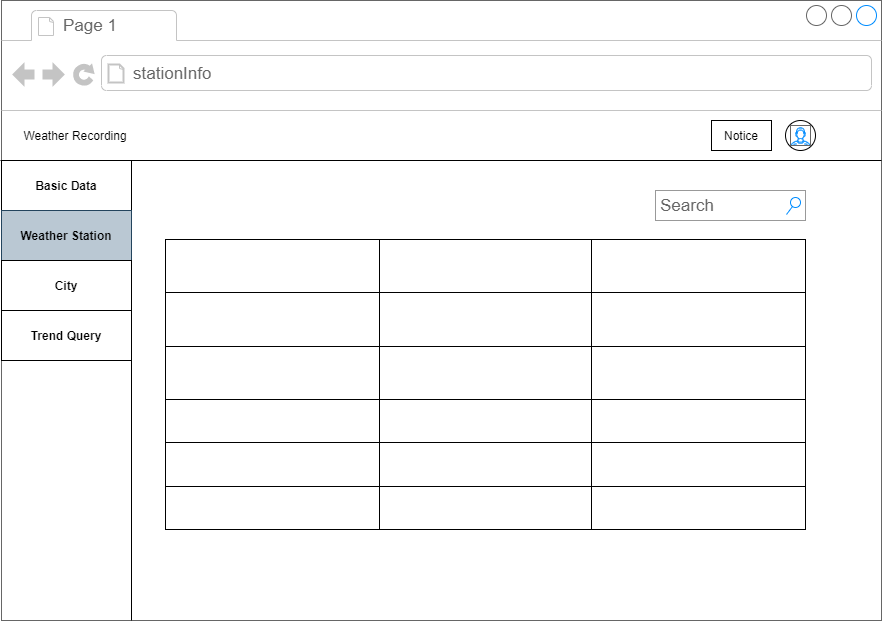
\includegraphics[width=0.8\linewidth]{../stationInfo}
		\caption{stationInfo}
		\label{fig:stationinfo}
	\end{figure}
	
	\noindent The city information web page can tell users about information of the cities from which we get the weather records.
	\begin{figure}[H]
		\centering
		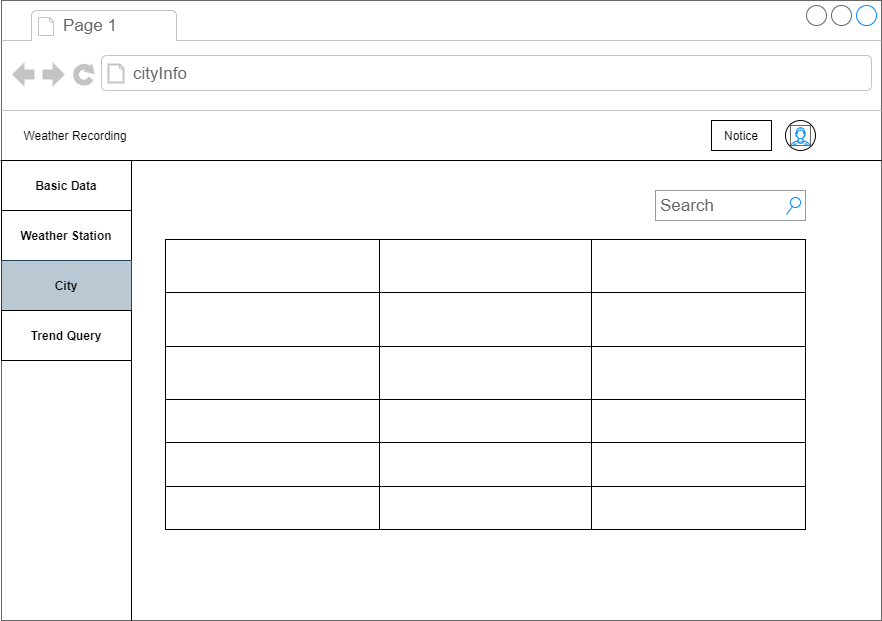
\includegraphics[width=0.8\linewidth]{../cityInfo}
		\caption{cityInfo}
		\label{fig:cityinfo}
	\end{figure}
	
	\noindent The Trend of Monthly Temperature web page is going to use the line chart to show the derived data of the basic data of temperature. User could choose from time and to time, which are all at the month time granularity. Users can also choose the certain weather station to get the data of the station. Users could figure out the changing of monthly temperature over the time period.
	\begin{figure}[H]
		\centering
		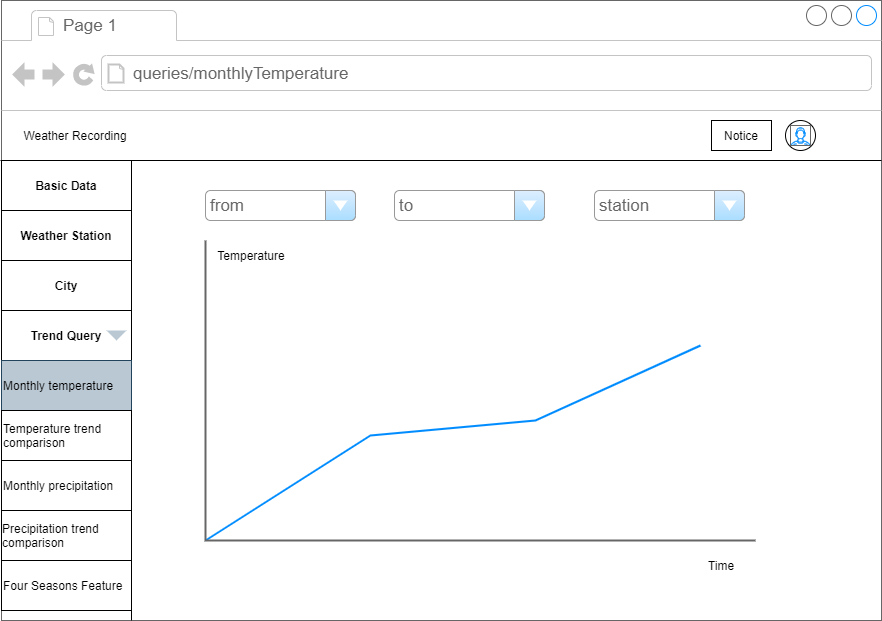
\includegraphics[width=0.8\linewidth]{../TrendOfTemperature}
		\caption{Monthly Temperature}
		\label{fig:trendoftemperature}
	\end{figure}

	\noindent The Trend of Temperature Comparison web page is going to use the line chart to show the difference of temperature between different cities. User could choose the certain year, and they can choose the cities they want to compare. Users could compare the temperature between several cities in the same year.
	\begin{figure}[H]
		\centering
		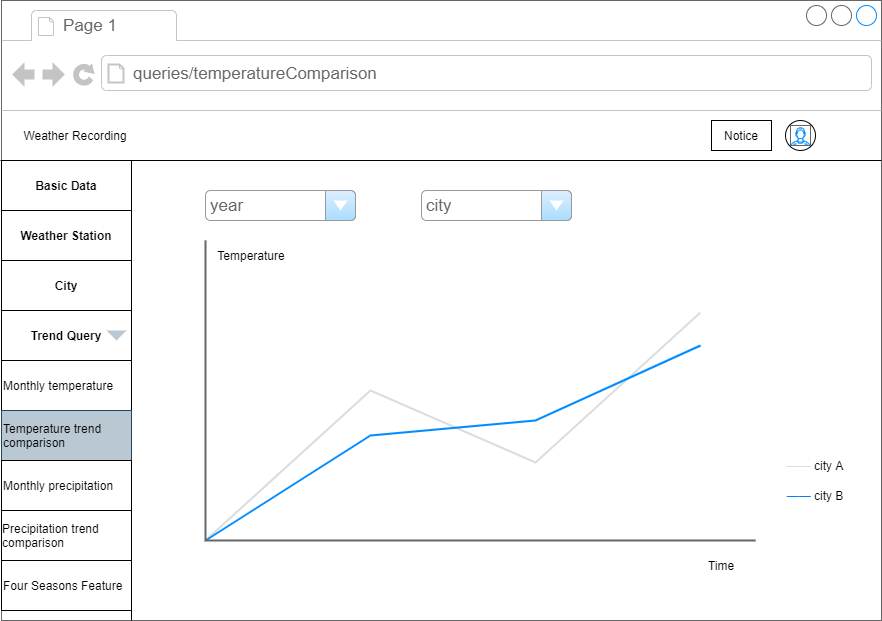
\includegraphics[width=0.8\linewidth]{../temperatureCompare}
		\caption{Temperature Compare}
		\label{fig:temperaturecompare}
	\end{figure}
	
	\noindent The Trend of Precipitation web page is going to use a bar chart to show the derived data of the basic data of precipitation. User could choose from time and to time, which are all at the month time granularity. Users can also choose the certain weather station to get the data of the station. Users could figure out the changing of monthly precipitation over the time period.
	\begin{figure}[H]
		\centering
		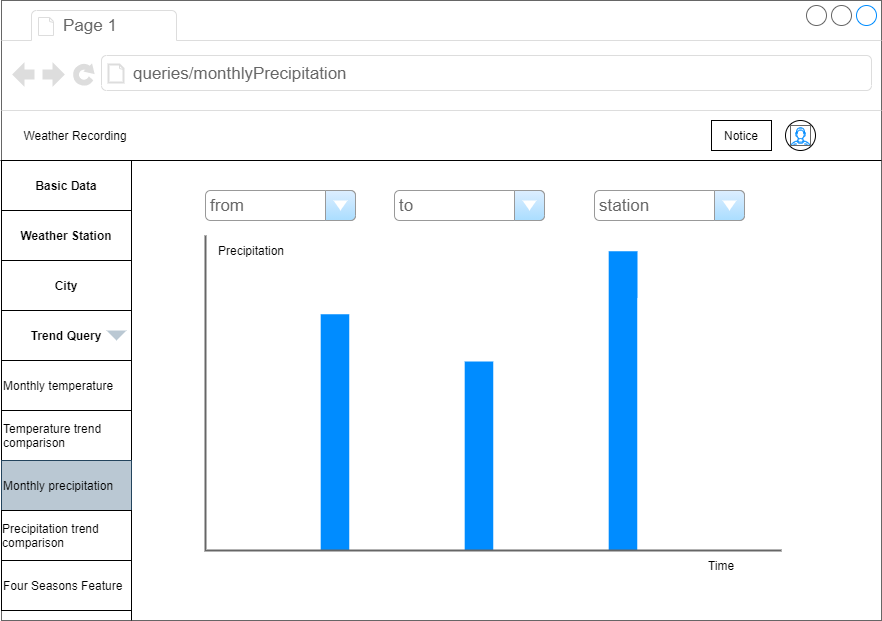
\includegraphics[width=0.8\linewidth]{../TrendOfPrecipitation}
		\caption{Monthly Precipitation}
		\label{fig:trendofprecipitation}
	\end{figure}
	
	\noindent The Trend of Precipitation Comparison web page is going to use the line chart to show the difference of precipitation between different cities. User could choose the certain year, and they can choose the cities they want to compare. Users could compare the precipitation between several cities in the same year.
	\begin{figure}[H]
		\centering
		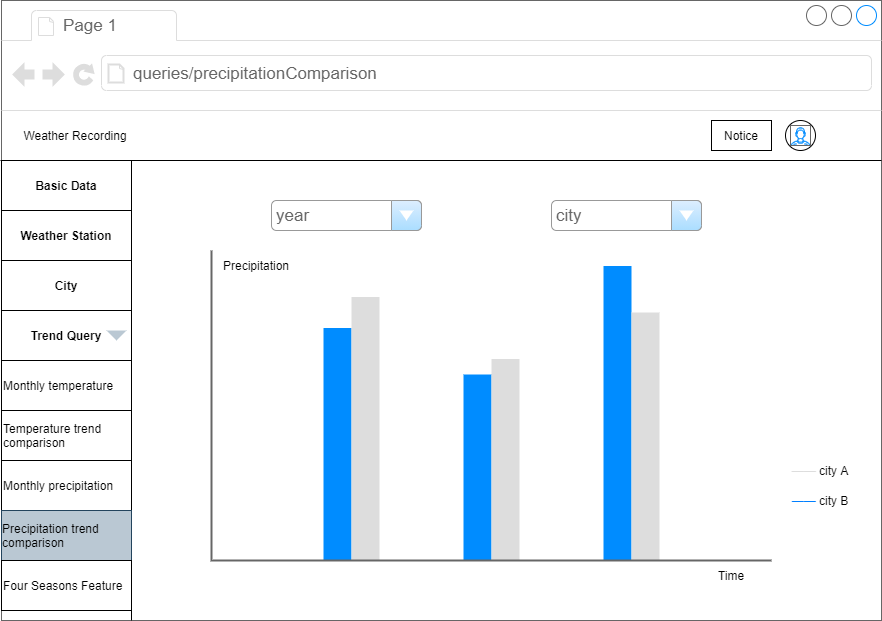
\includegraphics[width=0.8\linewidth]{../precipitationCompare}
		\caption{Precipitation Compare}
		\label{fig:precipitationcompare}
	\end{figure}
	
	\noindent The Trend of Four Seasons Feature web page is going to use two chart to figure out the features of four seasons of the city by showing temperature and precipitation of one year. User could choose the certain year, and they can choose only one city they want to know.
	\begin{figure}[H]
		\centering
		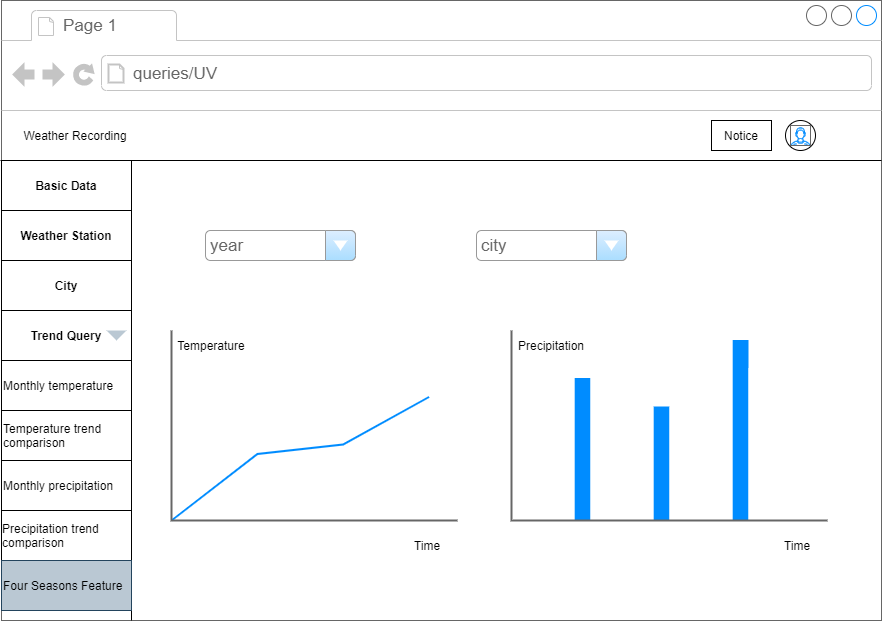
\includegraphics[width=0.8\linewidth]{../seasonsFeature}
		\caption{Seasons Feature}
		\label{fig:seasonsfeature}
	\end{figure}
	

	\subsection{Complex trend queries}
	
	\subsubsection{Trend of Monthly Temperature}
	
	\textbf{Description}  \\
	\noindent Users could learn about the trend of temperature change at different cities from our system. Users can choose the time period from one month to another month, they also need to choose one city to show the data. For example, users have to choose a time from '2020/08' to '2021/08', and the city 'Gainesville'. Then, the system will calculate the monthly average temperature of Gainesville from '2020/08' to '2021/08' according to the data sets. So, In the line chart, the x-axis is month and the y-axis is average temperature(Monthly).    \\
	
	\noindent \textbf{Integration into the web pages} \\
	\noindent The integration into the web page of Monthly Temperature is showed in Figure 10, the system provides the line chart to help user learn the temperature change.   \\
	
	\noindent \textbf{Output} \\
	\noindent The output of the Monthly Temperature query is data that contains time of month and the average temperature of the month.  
	
	\subsubsection{Trend of Temperature Comparison}

	\textbf{Description} \\
	\noindent Users could learn about the trend of temperature comparison between different cities from our system. Users can choose the year which they are concerned with, and they also need to choose at least two cities so that they could show the difference. For example, users will choose year 2020, then choose the city 'Gainesville' and 'Miami'. Then, the system will show two lines in the line chart and each curve is built by the average monthly temperature according to the data sets. So, In the line chart, the x-axis is month and the y-axis is average temperature(Monthly), but there are more than one lines.    \\

	\noindent \textbf{Integration into the web pages} \\
	\noindent The integration into the web page of Temperature Comparison is showed in Figure 11, the system provides the line chart to help user learn the camparison of different cities.    \\
	
	\noindent \textbf{Output} \\
	\noindent The output of the Temperature Comparison query is the data that contains city, time of month and the average temperature of the month over the choosen year.  
	
	\subsubsection{Trend of Monthly Precipitation}
	
	\textbf{Description} \\
	\noindent Users could learn about the trend of precipitation change at different cities from our system. Users can choose the time period from one month to another month, they also need to choose one city to show the data. For example, users have to choose a time from '2020/01' to '2020/12', and the city 'Tanpa'. Then, the system will calculate the monthly average temperature of Tanpa from '2020/01' to '2020/12' according to the data sets. So, In the bar chart, the x-axis is month and the y-axis is average precipitation(Monthly).    \\
	
	\noindent \textbf{Integration into the web pages} \\
	\noindent The integration into the web page of Monthly Precipitation is showed in Figure 12, the system provides the bar chart to help user learn the precipitation situation.    \\
	
	\noindent \textbf{Output} \\
	\noindent The output of the Monthly Precipitation query is data that contains time of month and the average precipitation of the month. 
	
	\subsubsection{Trend of Precipitation Comparison}
	
	\textbf{Description} \\
	\noindent Users could learn about the trend of precipitation comparison between different cities from our system. Users can choose the year which they are concerned with, and they also need to choose at least two cities so that they could show the difference. For example, users will choose year 2019, then choose the city 'Tanpa' and 'Miami'. Then, the system will show two different color bars in the bar chart and each bar is built by the average monthly precipitation according to the data sets. So, In the bar chart, the x-axis is month and the y-axis is average precipitation(Monthly), but there are different colors of bars.    \\
	
	\noindent \textbf{Integration into the web pages} \\
	\noindent The integration into the web page of Precipitation Comparison is showed in Figure 13, the system provides the line chart to help user learn the difference between precipitation of different cities.    \\
	
	\noindent \textbf{Output} \\
	\noindent The output of the Precipitation Comparison query is the data that contains city, time of month and the average precipitation of the month over the choosen year.  
	
	\subsubsection{Trend of Seasons Feature}
	
	\textbf{Description} \\
	\noindent Users could learn about the Seasons Feature at different cities from our system. Users can choose the certain year as well as the city to show the data. For example, users have to choose the year 2020, and the city 'Gainesville'. Then, the system will show two charts, one is the temperature chart and the other is precipitation chart. The user could figure out from the charts about whether the city has four distinctive seasons, or belongs to tropical climate.     \\
	
	\noindent \textbf{Integration into the web pages} \\
	\noindent The integration into the web page of Seasons Feature is showed in Figure 14, the system combine two charts to help user learn the feature of the seasons of the certain city.    \\
	
	\noindent \textbf{Output} \\
	\noindent The output of the Seasons Feature query is the data that contains two parts. The first part is the data of daily average temperature of the choosen year in order to show a curve of the temperature change, and the second part of the data is the average precipitation of each month during the year.
	
	\section{Quality of the conceptual database design based on the Entity-Relationship Model and a careful analysis of the deployed data sources}
	
	\begin{figure}[H]
		\centering
		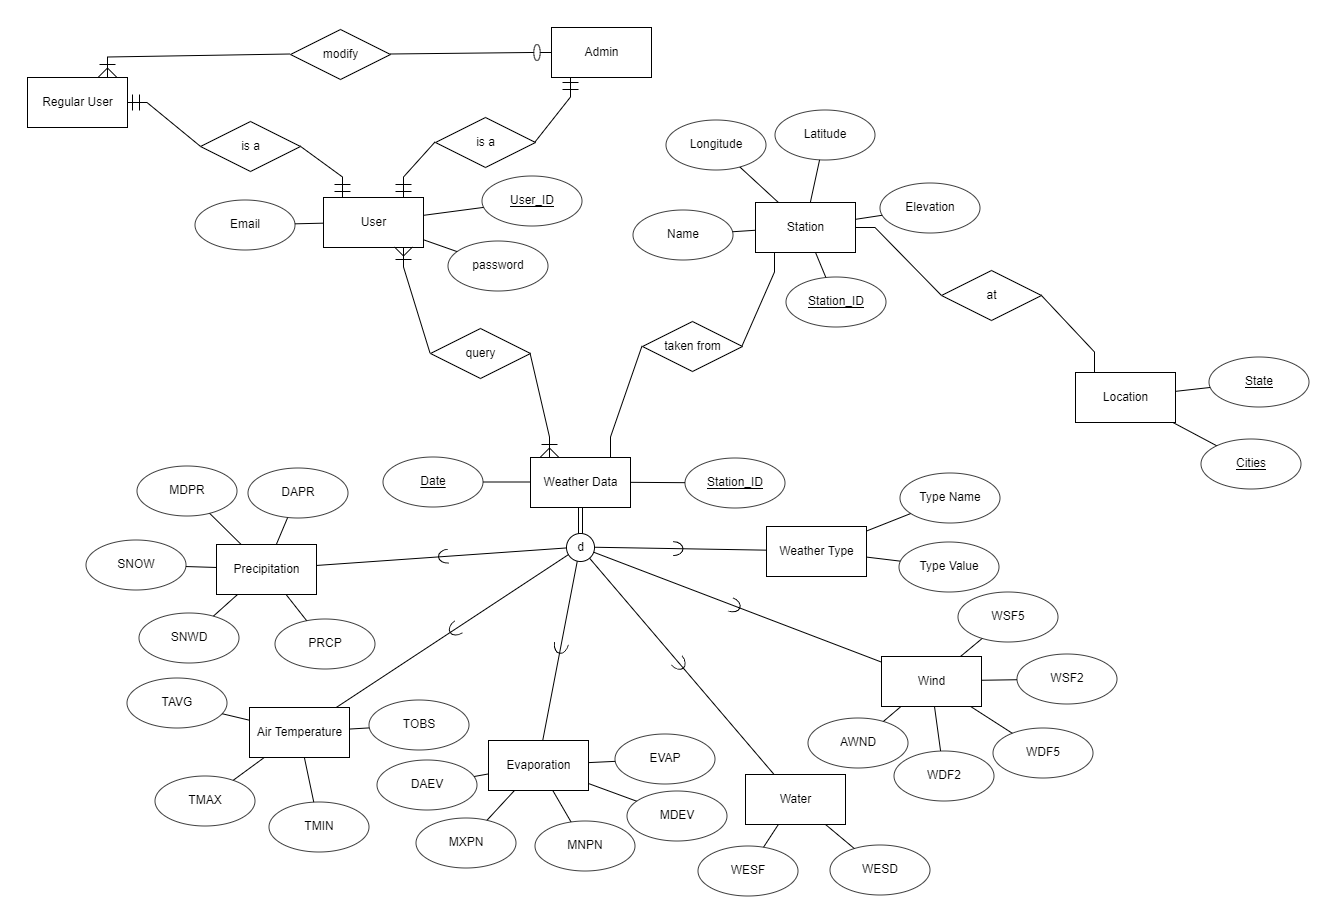
\includegraphics[width=1\linewidth]{../ER}
		\caption{ER-Diagram}
		\label{fig:er}
	\end{figure}
	
	According to the overall design of the system and the functional modules described above, we selected daily weather data from multiple cities from NOAA.gov. We selected a large number of data files based on the city name to construct the database to be used in the system. The data is selected by selecting cities, time periods and statistical methods. In this data set, the historical weather data of each city comes from weather stations in different locations in the city. For each weather station, it is determined by its name, and a detailed geographic location consisting of latitude, longitude and altitude. The data file composition of each city is roughly the same. According to our classification of entities, weather data can be classified into evaporation, precipitation, wind, air temperature, water, and weather types. \\
	
	\noindent Evaporation, which often used in meteorology to compare with precipitation. The comparative data is important to illustrate how dry and wet a place is. It includes attributes such as Daily maximum temperature of water in an evaporation pan (MXPN), Daily minimum temperature of water in an evaporation pan (MNPN), and Evaporation of water from evaporation pan (EVAP). The units of MXPN and MNPN are degrees Fahrenheit, and the unit of EVAP is inches. \\
	
	\noindent Precipitation refers to the depth of liquid or solid (melted) water that falls from the sky to the ground within a certain period of time, without evaporation, infiltration, or loss, but the depth that it accumulates on the horizontal surface. It includes the commonly used Multiday precipitation total (use with DAPR and DWPR, if available) (MDPR), Number of days included in the multiday precipitation total (MDPR) (DAPR), Precipitation (PRCP), Snow depth (SNWD), Snowfall (SNOW). The units of PRCP, SNWD and SNOW are all inches. \\
	
	\noindent Wind includes attributes like Average wind speed (AWND), Direction of fastest 2-minute wind (WDF2), Direction of fastest 5-second wind (WDF5), Fastest 2-minute wind speed (WSF2), Fastest 5-second wind speed (WSF5). The units of AWND, WSF2 and WSF5 are miles per hour, and the units of WDF2 and WDF5 are degrees.  \\
	
	\noindent Air temperature is composed of Average Temperature. (TAVG), Maximum temperature (TMAX), Minimum temperature (TMIN), Temperature at the time of observation (TOBS). Their units are all degrees Fahrenheit. In addition, we can easily calculate the temperature difference through TMAX and TMIN, which can be used as a derived attribute.   \\
	
	\noindent Water is mainly described by Water equivalent of snow on the ground (WESD), Water equivalent of snowfall (WESF), in inches.   \\
	
	\noindent The ‘**’ in Weather types (WT**) consists of several fixed values, and each value represents a different weather type. For details, please refer to the table below. \\
	
	\begin{table}[H]
		\begin{tabular}{|c|l|}
			\hline
			Value & \multicolumn{1}{c|}{Weather Type}                                      \\ \hline
			01    & Fog, ice fog, or freezing fog (may include heavy fog)                  \\ \hline
			02    & Heavy fog or heaving freezing fog (not always distinguished from fog)  \\ \hline
			03    & Thunder                                                                \\ \hline
			04    & Ice pellets, sleet, snow pellets, or small hail                        \\ \hline
			05    & Hail (may include small hail)                                          \\ \hline
			06    & Glaze or rime                                                          \\ \hline
			07    & Dust, volcanic ash, blowing dust, blowing sand, or blowing obstruction \\ \hline
			08    & Smoke or haze                                                          \\ \hline
			09    & Blowing or drifting snow                                               \\ \hline
			10    & Tornado, waterspout, or funnel cloud                                   \\ \hline
			11    & High or damaging winds                                                 \\ \hline
			12    & Blowing spray                                                          \\ \hline
			13    & Mist                                                                   \\ \hline
			14    & Drizzle                                                                \\ \hline
			15    & Freezing drizzle                                                       \\ \hline
			16    & Rain (may include freezing rain, drizzle, and freezing drizzle)        \\ \hline
			17    & Freezing rain                                                          \\ \hline
			18    & Snow, snow pellets, snow grains, or ice crystals                       \\ \hline
			19    & Unknown source of precipitation                                        \\ \hline
			20    & Ground fog                                                             \\ \hline
			21    & Fog, ice fog, or freezing fog (may include heavy fog)                  \\ \hline
		\end{tabular}
	\end{table}
	
	\noindent Select the weather data of Miami from October 1, 2020 to September 30, 2021 as a sample to show. The details are shown in the figure below. \\
	
	\begin{figure}[H]
		\centering
		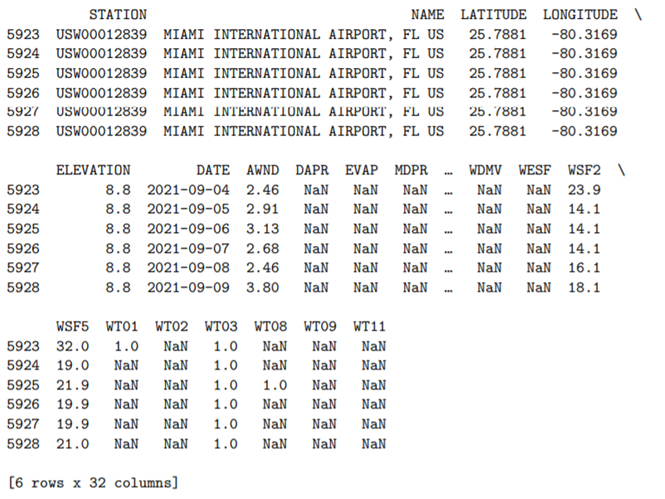
\includegraphics[width=0.5\linewidth]{../d2-p2-1}
		\caption{}
		\label{fig:d2-p2-1}
	\end{figure}
	
	\noindent Using tools such as pandas and numpy to conduct a simple analysis on this data set. It shows same basic information about the data set. Based on the data analysis, the required information can be used in subsequent specific implementations to enrich functions and optimize user experience. \\
	
	\begin{figure}[H]
		\centering
		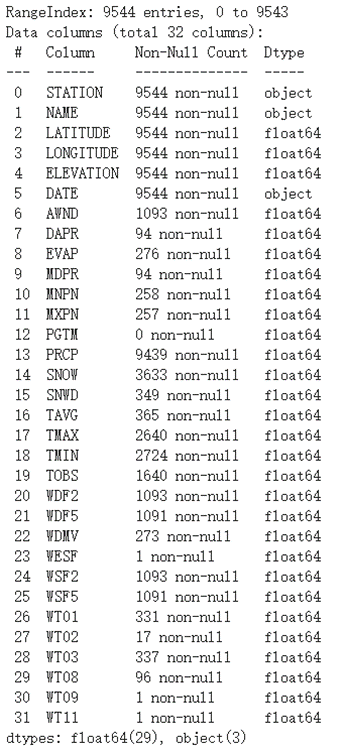
\includegraphics[width=0.6\linewidth]{../d2-p2-2}
		\caption{}
		\label{fig:d2-p2-2}
	\end{figure}
	
	
	\noindent This table shows the summary information of the selected data set. Including the number of entries, column names, and the count of non-empty entries for each column.  \\
	
	\begin{figure}[H]
		\centering
		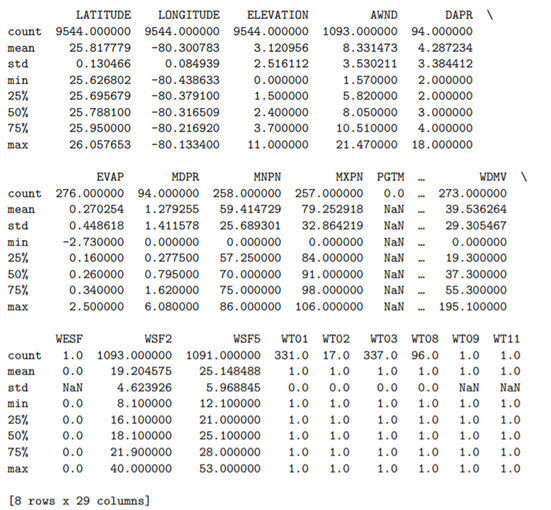
\includegraphics[width=0.7\linewidth]{../d2-p2-3}
		\caption{}
		\label{fig:d2-p2-3}
	\end{figure}
	
	\noindent For example, we can count the frequency of the daily maximum temperature (TMAX) in the area and display it in the form of graphs, which can furtherly help us analyze the trend of extreme temperature changes in a certain city.  \\
	\begin{figure}[H]
		\centering
		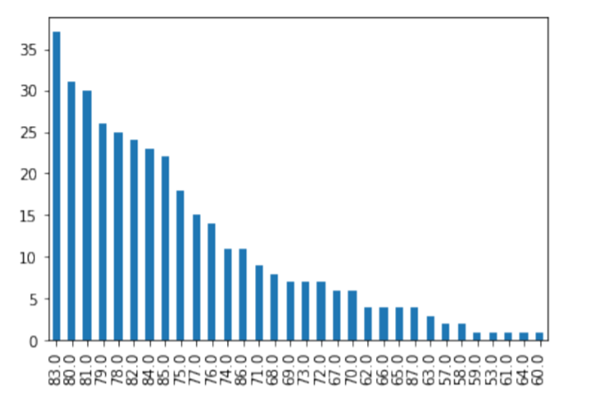
\includegraphics[width=0.7\linewidth]{../d2-p2-4}
		\caption{}
		\label{fig:d2-p2-4}
	\end{figure}
	
	
	
	
\end{document}
